\section{特殊角的三角函数}

\begin{adjustwidth}{2cm}{0cm}
    \begin{tikzpicture}[scale=4,x=1cm,y=1cm,>=stealth]
        \draw[->,blue,very thick](-1.5,0)--(1.5,0)node[above,red]{$ \cos\alpha$};
        \draw[->,blue,very thick](0,-1.5)--(0,1.5)node[above,red]{$ \sin\alpha$};
        \draw[blue,thick](0,0)circle(1);
        \draw[->,blue,very thick](-1.8,1)--(1.8,1)node[below,red]{$ \cot\alpha$};
        \draw[->,blue,very thick](1,-1.8)--(1,1.8)node[above,red]{$ \tan\alpha$};
        \draw[red,dotted,line width=1pt](30:1)rectangle(210:1)(45:1)rectangle(225:1) (60:1)rectangle(240:1);
        \draw[blue,dotted,line width=0.5pt](300:1)--(300:2) (315:1)--(315:1.4142)(330:1)--(330:1.1547)(30:1)--(30:2)(45:1)--(45:1.4142) (60:1)--(60:2)(120:1)--(120:1.1547)(135:1)--(135:1.4142)(150:1)--(150:2);
        \foreach\x in {0,30,45,60,90,120,135,150,180,210,225,240,270,300,315,330}
        \draw[green,dotted,line width=1pt](0,0)--(\x:1)node[scale=1,blue]{$ \bullet$} node[pos=1.125,scale=0.05,blue,fill=blue!10!white]{   $ $};
        \node at (0.94,0.5){\color{black}$ \dfrac{\pi}{6} $};
        \node at (0.79,0.75){\color{black}$ \dfrac{\pi}{4} $};
        \node at (0.59,0.9){\color{black}$ \dfrac{\pi}{3} $};
        \node at (-0.94,0.5){\color{black}$ \dfrac{5\pi}{6} $};
        \node at (-0.79,0.75){\color{black}$ \dfrac{3\pi}{4} $};
        \node at (-0.59,0.9){\color{black}$ \dfrac{2\pi}{3} $};
        \node at (0.94,-0.5){\color{black}$ \dfrac{-\pi}{6} $};
        \node at (0.79,-0.75){\color{black}$ \dfrac{-\pi}{4} $};
        \node at (0.59,-0.9){\color{black}$ \dfrac{-\pi}{3} $};
        \node at (-0.96,-0.5){\color{black}$ \dfrac{-5\pi}{6} $};
        \node at (-0.81,-0.75){\color{black}$ \dfrac{-3\pi}{4} $};
        \node at (-0.61,-0.9){\color{black}$ \dfrac{-2\pi}{3} $};
        \node at (1.05,0.1){\color{black}$ 0 $};
        \node at (0.1,1.15){\color{black}$ \dfrac{\pi}{2} $};
        \node at (-1.1,0.1){\color{black}$ \pi $};
        \node at (0.1,-1.15){\color{black}$ \dfrac{-\pi}{2} $};
        \draw[red,thick](0,0)node[scale=1,below left=0.05cm]{$ $};
        \draw[blue](300:2)node[right,scale=1]{$-\sqrt{3}$}(315:1.45)node[right,scale=1]{$1$}(328:1.15)node[right,scale=1]{$\dfrac{-1}{\sqrt{3}}$}(33:1.16)node[right,scale=1]{$ \dfrac{-1}{\sqrt{3}}$}(30:2)node[above,scale=1]{$ \sqrt{3}$}(45:1.45)node[above right,scale=1]{$ 1$}(60:2)node[right,scale=1]{$ \sqrt{3}$}
        (62:1.11)node[above right,scale=1]{$ \dfrac{1}{\sqrt{3}}$}(118:1.12)node[above left,scale=1]{$ \dfrac{-1}{\sqrt{3}}$}
        (134:1.41)node[above left,scale=1]{$ -1$}(150:2)node[above,scale=1]{$ -\sqrt{3}$};
        \draw[blue](-0.89,0)node[below,scale=.7]{$ \dfrac{-\sqrt{3}}{2}$}(-0.72,0)node[below,scale=.7]{$ \dfrac{-\sqrt{2}}{2}$}(-0.52,0)node[below,scale=.7]{$ \dfrac{-1}{2}$}(0.865,0)node[below,scale=.7]{$\dfrac{\sqrt{3}}{2}$}(0.7065,0)node[below,scale=.7]{$\dfrac{\sqrt{2}}{2}$}(0.5,0)node[below,scale=.7]{$\dfrac{1}{2}$}(0,-0.865)node[right,scale=.7]{$ \dfrac{-\sqrt{3}}{2}$}(0,-0.695)node[right,scale=.7]{$ \dfrac{-\sqrt{2}}{2}$}(0,-0.5)node[right,scale=.7]{$ \dfrac{-1}{2}$}(0,0.885)node[right,scale=.7]{$\dfrac{\sqrt{3}}{2}$}(0,0.7065)node[right,scale=.7]{$\dfrac{\sqrt{2}}{2}$}(0,0.517)node[right,scale=.7]{$\dfrac{1}{2}$};
    \end{tikzpicture}
\end{adjustwidth}

\begin{table}[H]
    \centering
    \caption{特殊角三角函数值 (0\si{\degree} \~ 360\si{\degree})}
    \label{tab:special_angles_split}
    \renewcommand{\arraystretch}{1.5}

    % --- 左侧表格 (0° -- 90°) ---
    \begin{tabular}{ S[table-format=3] c c c c }
        \toprule
        \multicolumn{1}{c}{\textbf{角度 $\boldsymbol{\alpha}$}} &
        \textbf{弧度 $\boldsymbol{\theta}$}                     &
        $\boldsymbol{\sin\theta}$                             &
        $\boldsymbol{\cos\theta}$                             &
        $\boldsymbol{\tan\theta}$                                                                                                                     \\
        \midrule
        \SI{0}{\degree}                                       & $0$              & $0$                  & $1$                  & $0$                  \\
        \SI{30}{\degree}                                      & $\frac{\pi}{6}$  & $\frac{1}{2}$        & $\frac{\sqrt{3}}{2}$ & $\frac{\sqrt{3}}{3}$ \\
        \SI{45}{\degree}                                      & $\frac{\pi}{4}$  & $\frac{\sqrt{2}}{2}$ & $\frac{\sqrt{2}}{2}$ & $1$                  \\
        \SI{60}{\degree}                                      & $\frac{\pi}{3}$  & $\frac{\sqrt{3}}{2}$ & $\frac{1}{2}$        & $\sqrt{3}$           \\
        \SI{90}{\degree}                                      & $\frac{\pi}{2}$  & $1$                  & $0$                  & 不存在                  \\
        \SI{120}{\degree}                                     & $\frac{2\pi}{3}$ & $\frac{\sqrt{3}}{2}$ & $-\frac{1}{2}$       & $-\sqrt{3}$          \\
        \bottomrule
    \end{tabular}
    \quad
    \begin{tabular}{ S[table-format=3] c c c c }
        \toprule
        \multicolumn{1}{c}{\textbf{角度 $\boldsymbol{\alpha}$}} &
        \textbf{弧度 $\boldsymbol{\theta}$}                     &
        $\boldsymbol{\sin\theta}$                             &
        $\boldsymbol{\cos\theta}$                             &
        $\boldsymbol{\tan\theta}$                                                                                                                       \\
        \midrule
        \SI{135}{\degree}                                     & $\frac{3\pi}{4}$ & $\frac{\sqrt{2}}{2}$ & $-\frac{\sqrt{2}}{2}$ & $-1$                  \\
        \SI{150}{\degree}                                     & $\frac{5\pi}{6}$ & $\frac{1}{2}$        & $-\frac{\sqrt{3}}{2}$ & $-\frac{\sqrt{3}}{3}$ \\
        \SI{180}{\degree}                                     & $\pi$            & $0$                  & $-1$                  & $0$                   \\
        \SI{210}{\degree}                                     & $\frac{7\pi}{6}$ & $-\frac{1}{2}$       & $-\frac{\sqrt{3}}{2}$ & $\frac{\sqrt{3}}{3}$  \\
        \SI{270}{\degree}                                     & $\frac{3\pi}{2}$ & $-1$                 & $0$                   & 不存在                   \\
        \SI{360}{\degree}                                     & $2\pi$           & $0$                  & $1$                   & $0$                   \\
        \bottomrule
    \end{tabular}
\end{table}